\documentclass{report}
\usepackage{fullpage}
\usepackage{graphicx}
\usepackage{array}
\usepackage{float}
\usepackage{titlesec}

\titleformat{\section}
  {\large\bfseries\centering} % Font style and size
  {\thesection}     % Section number
  {1em}             % Space between number and title
  {}                % Code before the title


\renewcommand{\baselinestretch}{2}
% Redefine the title page
% Redefine the title page
\makeatletter
\renewcommand{\maketitle}{
    \begin{titlepage}
        \centering
        \vspace*{2cm}

        {\LARGE \bfseries \@title \par}
        \vspace{1.5cm}
        {\Large \@author \par}
        
        { Entry Number: 2024AIM1011 \par}
        \vspace{-0.3cm}
        {Course Code: CS506 \par}
        {\Large Department of Computer Science and Engineering \par}
        \vspace{2cm}
        
        \vfill
    \end{titlepage}
}
\makeatother

\author{Yash Narnaware}
\title{Analysis of median of medians for Quicksort}
\begin{document}




\maketitle

\renewcommand{\arraystretch}{0.6}


\setlength{\tabcolsep}{2pt}

\section*{Array sizes vs time for different implementations of Quicksort}
I have generated arrays of different sizes with random values to see how each implementation - normal quicksort and quicksort using medians of medians for different subarray intervals like 3, 5, and 7 performs on it.

Here are the testing results - 

\begin{table}[H]
\centering
\footnotesize
\begin{tabular}{|c|c|c|c|c|}
\hline
\textbf{Array Size} & \textbf{Normal Quicksort} & \textbf{MoM3 Quicksort} & \textbf{MoM5 Quicksort} & \textbf{MoM7 Quicksort} \\ \hline
100   & 0.00001  & 0.000029  & 0.000021  & 0.000022  \\ \hline
200   & 0.000013 & 0.000041  & 0.000043  & 0.000051  \\ \hline
400   & 0.00003  & 0.000088  & 0.000098  & 0.000144  \\ \hline
800   & 0.000061 & 0.000203  & 0.000286  & 0.000274  \\ \hline
1600  & 0.000152 & 0.000483  & 0.00054   & 0.000547  \\ \hline
3200  & 0.000287 & 0.000927  & 0.001053  & 0.00113   \\ \hline
6400  & 0.000518 & 0.001964  & 0.002296  & 0.002503  \\ \hline
12800 & 0.001161 & 0.004204  & 0.00492   & 0.005363  \\ \hline
15000 & 0.001351 & 0.004865  & 0.005802  & 0.006317  \\ \hline
18000 & 0.001638 & 0.006019  & 0.007117  & 0.007847  \\ \hline
20000 & 0.001812 & 0.006785  & 0.007956  & 0.008727  \\ \hline
22000 & 0.002002 & 0.007509  & 0.008859  & 0.009775  \\ \hline
25600 & 0.002348 & 0.008753  & 0.010457  & 0.011541  \\ \hline
28000 & 0.0026   & 0.009676  & 0.011621  & 0.012631  \\ \hline
35000 & 0.003306 & 0.012392  & 0.01479   & 0.016258  \\ \hline
50000 & 0.005137 & 0.018781  & 0.021746  & 0.023783  \\ \hline
\end{tabular}
\caption{Time(in seconds) taken by various implementations of quicksort for randomly generated arrays}
\label{table:quicksort_comparison}
\end{table}

\begin{figure}[H]
\centering
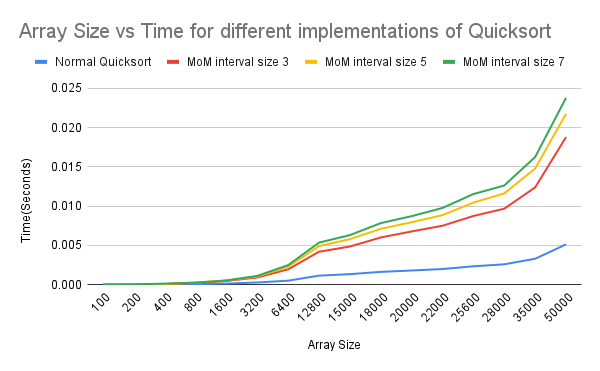
\includegraphics[scale=0.6]{sizevstime.png}

\end{figure}


By looking at the test results, I don't think selecting pivot using median will help in this case because our array elements are in random order, and in normal quicksort we are selecting the starting element (which can be the last element or any other element) to be pivot, and there is a very small chance of this chosen pivot to be at the extreme ends of the array. That's why normal quicksort is performing well when data is in random order, because in other implementations, choosing pivot is adding extra time.



\section*{Sorted array vs time for different implementations of Quicksort}

In this case the generated arrays are already in sorted order lets see how different algorithms performs on it.

\begin{table}[H]
\centering
\footnotesize % Optional: Use \footnotesize or \scriptsize to make the table smaller
\begin{tabular}{|c|c|c|c|c|}
\hline
\textbf{Array Size} & \textbf{Normal Quicksort} & \textbf{MoM3 Quicksort} & \textbf{MoM5 Quicksort} & \textbf{MoM7 Quicksort} \\ \hline
100    & 0.00002  & 0.00004  & 0.000023 & 0.000023 \\ \hline
200    & 0.000049 & 0.000081 & 0.000078 & 0.000047 \\ \hline
400    & 0.000168 & 0.000353 & 0.000115 & 0.000154 \\ \hline
800    & 0.000586 & 0.000741 & 0.000532 & 0.000239 \\ \hline
1600   & 0.001907 & 0.00177  & 0.00084  & 0.000489 \\ \hline
3200   & 0.007506 & 0.007707 & 0.002112 & 0.002287 \\ \hline
6400   & 0.017208 & 0.009767 & 0.00415  & 0.003012 \\ \hline
12800  & 0.066929 & 0.036061 & 0.009764 & 0.004738 \\ \hline
15000  & 0.095404 & 0.042685 & 0.010342 & 0.006383 \\ \hline
18000  & 0.143551 & 0.051646 & 0.019739 & 0.012501 \\ \hline
20000  & 0.166875 & 0.073927 & 0.036015 & 0.021332 \\ \hline
22000  & 0.202082 & 0.096411 & 0.034407 & 0.024358 \\ \hline
25600  & 0.270739 & 0.117527 & 0.033535 & 0.023083 \\ \hline
28000  & 0.318364 & 0.158395 & 0.036345 & 0.023416 \\ \hline
35000  & 0.53649  & 0.197357 & 0.047864 & 0.038278 \\ \hline
50000  & 1.110989 & 0.316686 & 0.062427 & 0.047158 \\ \hline
\end{tabular}
\caption{Time(in seconds) taken by various implementations of quicksort when arrays are sorted}
\label{table:quicksort_comparison_2}
\end{table}

Plotting the above data - 


\begin{figure}[H]
\centering
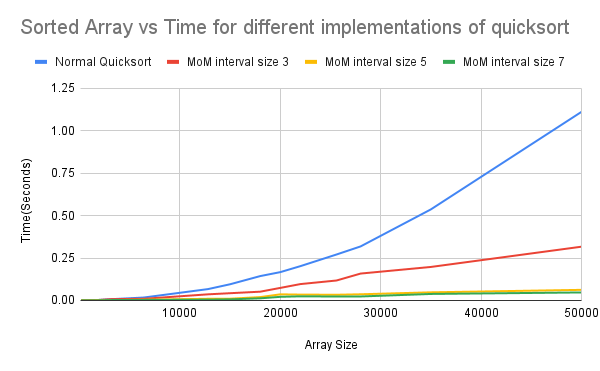
\includegraphics[scale=0.6]{sortedvstime.png}

\end{figure}

It is apparent from the figure that the median of medians implementation is performing better than normal quicksort when the arrays are sorted, and it should be the case because when arrays are sorted, normal quicksort will choose the first element of the array as a pivot (commonly used pivot), and since it is sorted, the array pivot will be the smallest element, and it will divide the array in the worst possible way while partitioning. That's why the median of medians is performing better than normal quicksort in this case.

\newpage
\section*{Reverse sorted array vs time for different implementations of Quicksort}

In this case the generated arrays are in reverse sorted order lets see how different algorithms performs on it.


\begin{table}[H]
\centering
\footnotesize % Optional: Use \footnotesize or \scriptsize to make the table smaller
\begin{tabular}{|c|c|c|c|c|}
\hline
\textbf{Array Size} & \textbf{Normal Quicksort} & \textbf{MoM interval size 3} & \textbf{MoM interval size 5} & \textbf{MoM interval size 7} \\ \hline
100    & 0.000016 & 0.000035 & 0.00002  & 0.00005  \\ \hline
200    & 0.000044 & 0.000066 & 0.000061 & 0.000038 \\ \hline
400    & 0.000182 & 0.000234 & 0.00007  & 0.000099 \\ \hline
800    & 0.000493 & 0.000292 & 0.000253 & 0.000186 \\ \hline
1600   & 0.001541 & 0.000622 & 0.000438 & 0.000329 \\ \hline
3200   & 0.006736 & 0.002567 & 0.001116 & 0.001277 \\ \hline
6400   & 0.023793 & 0.005096 & 0.003166 & 0.002486 \\ \hline
12800  & 0.095172 & 0.019431 & 0.00687  & 0.004293 \\ \hline
15000  & 0.132961 & 0.019898 & 0.006951 & 0.005196 \\ \hline
18000  & 0.193165 & 0.027736 & 0.016051 & 0.010534 \\ \hline
20000  & 0.24487  & 0.036812 & 0.023892 & 0.016414 \\ \hline
22000  & 0.275811 & 0.047695 & 0.024659 & 0.017187 \\ \hline
25600  & 0.372535 & 0.059822 & 0.025531 & 0.018521 \\ \hline
28000  & 0.449816 & 0.07757  & 0.027673 & 0.019388 \\ \hline
35000  & 0.555333 & 0.201452 & 0.045225 & 0.026151 \\ \hline
50000  & 1.095356 & 0.273307 & 0.047955 & 0.044183 \\ \hline
\end{tabular}
\caption{Time(in seconds) taken by various implementations of quicksort when arrays are reverse sorted}
\label{table:quicksort_comparison_3}
\end{table}

\begin{figure}[H]
\centering
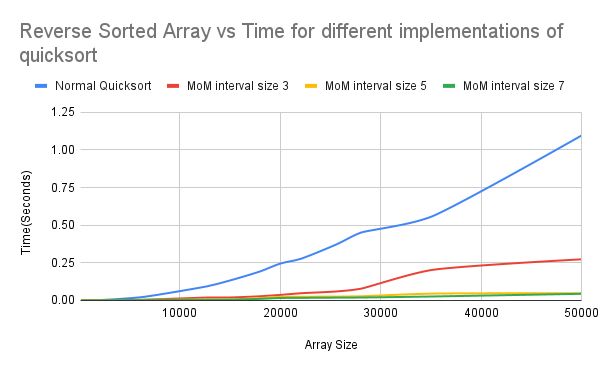
\includegraphics[scale=0.6]{reversesortedvstime.png}

\end{figure}

Again, like in the in the last case, normal quicksort will take the largest element in the first iteration as a pivot, then the second largest in the second iteration as a pivot, and so on, and it is the worst possible pivot for quicksort. That's why a similar trend follows as in the last case (sorted arrays).


\section*{Number of comparisons vs array size for different implementations of Quicksort}

I generated arrays of different sizes with random values to see the number of comparisons done by each algorithm.


\begin{table}[H]
\centering
\footnotesize % Optional: Use \footnotesize or \scriptsize to make the table smaller
\begin{tabular}{|c|c|c|c|c|}
\hline
\textbf{Array Size} & \textbf{Normal Quicksort} & \textbf{MoM interval size 3} & \textbf{MoM interval size 5} & \textbf{MoM interval size 7} \\ \hline
100    & 807     & 615     & 564     & 544     \\ \hline
200    & 1555    & 1324    & 1326    & 1355    \\ \hline
400    & 3588    & 3083    & 3031    & 3003    \\ \hline
800    & 9150    & 7009    & 6973    & 6912    \\ \hline
1600   & 20694   & 15711   & 15506   & 15148   \\ \hline
3200   & 44919   & 35525   & 34086   & 33510   \\ \hline
6400   & 99051   & 76650   & 75009   & 73805   \\ \hline
12800  & 206349  & 165904  & 163910  & 160728  \\ \hline
15000  & 272115  & 197651  & 196179  & 191719  \\ \hline
18000  & 336377  & 243875  & 238315  & 234861  \\ \hline
20000  & 363938  & 272597  & 267773  & 264708  \\ \hline
22000  & 380950  & 303997  & 297486  & 295606  \\ \hline
25600  & 454220  & 360008  & 353247  & 350174  \\ \hline
28000  & 504367  & 397223  & 388335  & 385554  \\ \hline
35000  & 653098  & 511141  & 499465  & 493713  \\ \hline
50000  & 999347  & 758572  & 741104  & 735353  \\ \hline
\end{tabular}
\caption{Number of comparisons for different array sizes}
\label{table:quicksort_execution_times}
\end{table}

\begin{figure}[H]
\centering
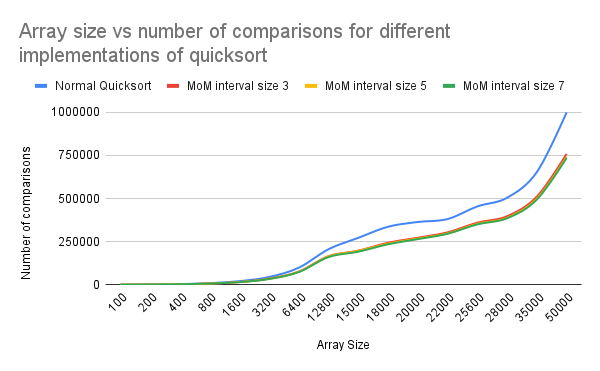
\includegraphics[scale=0.6]{numberofcomparisons.png}

\end{figure}


By looking at the data we can conclude that choosing a good pivot reduces the number of comparisons.

\newpage
\section*{Conclusion}


When the array elements are in random order, normal quicksort is performing the best, followed by the median of medians with sub-array interval 3, then sub-array interval 5, and then 7. In all the other cases, normal quicksort is the worst-performing algorithm, and the performance of MoM sub-array size 3 is worse than MoM sub-array sizes 5 and 7. MoM sub-array size 7 is better than MoM sub-array size 5 by a small margin. The number of comparisons for normal quicksort is greater than all 3 other implementations, and the number of comparisons for all 3 medians of the medians algorithm is similar.
































\end{document}